\documentclass[9pt]{article}
\title {Logistic maps for Coronavirus modeling}

\usepackage{graphicx}
\usepackage{verbatim}
\usepackage{amsthm}
\usepackage{amssymb}
\usepackage{amsmath}
\newtheorem{deff}{Definition}

\newcommand{\norm}[1]{\left\lVert#1\right\rVert}
\newtheorem{theorem}{Proposition}
\newtheorem{definition}{Definition}

\begin{document}
\maketitle
\section{Introduction}
A goal in modeling Coronavirus spreading is to find the function
$Y(t)$ describing the number of infected in time.
One need to assume the belonging of $Y$ to some family of functions
described by $n$ real parameters, estimating them after the observation
of empirical measurements subjected to noise.


By collecting the parameters into a vector $P \in \mathbb{R}^n$, 
we stress these dependence by writing $Y(t) = Y^P(t)$ when needed.


We start by recalling how many epidemiological models are member of 
the family of autonomous ODEs. This is for instance the case of
SIS (and their related), as well as of general logistic maps.
After pointing out a connection between these two common classes,
we explain in detail our choice in favor of the basic logistic map,
the Gompertz
law and the Richard ODE. In other words,
we assume $Y^P(t)$ to be always a logistic
curve described as solution of an autonomous 1-dimensional ODE 
depending on parameters $P$.


As an effective strategy to perform interpolation from noised data,
we suggest the use of Bayesian Inversion methods, 
a probabilistic viewpoint capable of managing errors naturally.


Before moving on concrete predictions for Germany and Italy,
we remark how important is the choice of the day zero on which to start
the model's dynamic. Indeed, the semigroup property of the flow
must be respected. It reflects the intuitive idea that countermeasure
policies may be not constant in time.

\section {The use of logistic models}
\subsection {Introduction}
One of the simplest idea for epidemiological modeling is to divide the
number of total existing people $N$, 
into two classes $S(t)$ and $I(t)$, such that
their sum $S + I = N$ is constant over time. People switch dynamically from
the set $S$ of \emph{susceptible}, to $I$ of \emph{infected}, and
conversely. Observe how in this model there are no fatal cases,
but this does not represent a problem since we take it just as a
starting point.
This simple scheme is known under the name of SIS and
governed by a system of two ODEs:

\begin{equation}
\begin{cases}
	S'(t) = - \beta S(t) I(t) + \alpha I(t) \\
	I'(t) = - \alpha I(t) + \beta S(t) I(t) \\
\end{cases}
\end{equation}


A complete explanation about the interpretation and the ideas beyond can be
found in REF, but for us it now important to remark how $\beta$ and $\alpha$
have specific interpretations. Beta is connected to how many 
people randomly meet per unit of time,
while $\frac{1}{\alpha}$ is the mean time required to heal. 


Since the sum $S + I = N$ is constant over time, a substitution
into the ODE leads to the simple logistic equation governing the number of
actively infected:

\begin{equation}
	I' (t) = r I(t) \left (1 - \frac{1}{K} \right)
\end{equation}
where $r = \beta N - \alpha$ and $k = N - \frac{\alpha}{\beta}$.


The equation above belongs to the family of logistic functions, maps
in principle not specifically connected to epidemiology. They are curves
obtained as solution of one dimensional
autonomous ODEs, with S-shaped trajectories starting with an exponential
growth, gradually stopped, until reaching an horizontal constant phase.


We chosen them as a prototype model for our simulations,
justified by the intuition that if the simplest compartmental
epidemiology model (SIS) is equivalent to the simplest logistic map,
then by choosing more general logistic functions we might implicitly
work with more realistic epidemiological models.


We furthermore do not just model the number of actively infected,
but rather use the equations to estimate the number of total infected
as well as of fatal cases.

We ignore further theoretical explanation for this decision,
but we simply
kept our choice encouraged by promising concrete results.

\subsection {The generalized logistic map}
The most general logistic map still expressed by an ODE
(we'll see later the reason beyond this requirement)
is given by the Richard's equation.
It's the following ordinary differential equation governed by
three real positive parameters, 
$P = \{ q, Q, \nu \}$. We need to fix an initial condition $Q_0$
(not considered as parameter since directly observed from data),
and we'll write the model as $Y(t) = Y^P(t) = Y^P_{Q_0}(t)$
when we want to stress this dependence.


The general logistic maps is the equation:

\begin{equation}
	Y'(t) = q Y(t) 
	\left ( 1 - \left( \frac{Y(t)}{Q} \right)^{\nu}\right )
\end{equation}
with closed form solution:
\begin{equation}
	Y(t) = \frac{Q} { (1 + A \exp[-q \nu t])^{\frac{1}{\nu}}}
\end{equation}

Here $A$ is just an abbreviation  for
$A = -1 + \left ( \frac{Q} { Q_0} \right )^{\nu}$.


The parameter $\nu$ is related to the symmetry of the curve,
while $p$ represents the initial exponential growth then stopped
in time. Intuitively speaking, we think of it to be related to the
average amount of people's social contact, as in the simpler logistic case
connected to the SIS model.


Note that by taking the limit $\lim_{t \to \infty} Y(t) = Q$, 
we understand how to read $Q$ as the asymptotic number of infected.


By setting $\nu = 1$ we obtain the basic logistic map, described
in the next section, while by taking the limit $\nu \mapsto 0$ 
under appropriate
hypothesis we get the Gompertz law, explained later.



\subsection {The simple logistic map}
In the simple logistic map the model $Y^P(t)$ depends on two real positive
parameters, $P = \{ q, Q \}$ and is the solution of the 1-dimensional ODE:
\begin{equation}
	Y'(t)  = q Y(t) \left ( 1 - \frac{Y(t)}{Q} \right )
\end{equation}
with closed-form formula:
\begin{equation}
Y(t) = \frac{Q_0 \exp[q t]}
	{1-\frac{Q_0}{Q} (1-\exp[q t)])}
\end{equation}


Where again $Q_0$ is the starting ODE condition at time $0$.
Of course, we have $\lim_{t \to \infty} Y(t) = Q$,
and since this simple logistic map is equivalent to the simplest SIS
model (as explained before), the parameter $q$ can be actually
rigorously related to the average number of daily people's social interaction.


\subsection{The Gompertz law}
The Gompertz law is governed by two real positive parameters,
$q$ and $Q$, therefore we write again $P = \{q, Q\}$.
Once the starting condition $Q_0$ at time zero
is specified, $Y(t) = Y^P(t) = Y_{Q_0}^P(t)$ is the solution to:

\begin{equation}
 Y'(t) = q Y(t) \log \left [\frac{Q} {Y(t)} \right ]
\end{equation}
expressed by the closed-form formula:
\begin{equation}
Y(t) = Q \exp	\left [
	\log \left [ \frac{Q_0}{Q} \right ]
	\exp \left [ -q t \right ]
		\right ]
\end{equation} 


As seen for the previous cases, too, $Q$ is also the limit
$\lim_{t \to \infty} Y(t)$.
Finally, note that we used always the same notation $P$ for all the models
described. This is because the techniques explained later apply equally
to all the cases above. When we make predictions, we'll have separate sections
for each models leaving no space for ambiguity.


Now that the models are hopefully clear, we move on explaining how we
intend to deduce the best values of $P$ starting from noised datasets.

\section {The Bayesian approach}
\subsection {Inverse Bayesian problems}
As a general formulation, the inverse problem 
consists on having a known borelian \emph{observation operator}
$G: \mathbb{R}^n \to \mathbb{R}^m$, an \textbf{unknown} 
input $x \in \mathbb{R}^n$ to be found from
a known \emph{measurement} $y = G(x) + \eta$, where $\eta$ is a centered
gaussian random variable, called the noise, with some specified variance.
With an abuse of notation we indicate with $\eta$ its gaussian
density function, too, therefore writing 
$\eta(u), u \in \mathbb{R}^m$ will be meaningful.


In other words we are interested in performing an indirect estimation 
(the value $x$) from a noised direct measurement $y$
through the use of a model $G$.
A \emph{lot} of theoretical issues are here into play. To mention
few of them, the map $G$ might admit different preimages, none at all,
or the noise might send $y$ outside the range of $G$.
Some of these problems are circumvented by minimizing appropriate distances
$\norm{G(x) - y}$ instead, but they might be insufficient or too hard.


In support on the described challenge,
switching to a probabilistic mindset can offer a precious support.
Simply observe the conditioned distribution induced from the noise:
\begin{equation}
	\mathbb{P} [ y | x] = \eta(y - G(x))
\end{equation}

The probability measure above is called the \emph{likelihood} and is
the key point of our reasoning. This is simply a gaussian centered on the true
value of $x$.
When the variance is small, the probabilistic search for $x$ 
is a relatively easy process, being $x$ the unique solution
that maximizes the probability.
But when the noise is increased,
the bell enlarges making harder to distinguish the "true" $x$
from points in its neighborhoods, who share now very high
probability values.
Theoretically $x$ is still unique, but in practice the interval
of uncertainty is much larger.

In the bayesian approach we start from these remarks,
but we also suppose to have a belief about the true value of $x$,
by choosing a probability distribution $\rho$ on the domain
$\mathbb{R}^n$ called the
\emph{prior}.
Then we rely on the Bayes formula:

\begin{equation}
\mathbb{P}[x | y] = \frac{ \mathbb{P}[y | x] \mathbb{P}[x]} {\mathbb{P}[y]}
\end{equation}

to define the \emph{posterior} distribution, still on the domain
$\mathbb{R}^n$, as:
\begin{equation}
\mu (x) \doteq \mathbb{P}[x|y] = \frac{ \eta(y - G(x)) \rho(x)} {\mathbb{P}[y]}
\end{equation}


Since the point $y$ is fixed, the denominator is just the normalization
constant than we can ignore thanks to suitable numerical methods.


The measure $\mu$ is the mathematically
formalization of the idea: "the best that we can say (about $x$) starting
from a certain belief ($\rho$) and (noised) concrete observations ($y$)".


We define $\mu$ to be the solution of the inversion problem.
Its statistical properties will say a lot about the uncertainty around
the true input $x$.


\subsection{The pCN Monte Carlo algorithm}
In the previous section we explained how we converted the problem of
an input reconstruction, to the problem of understating a probability
measure $\mu$ on $\mathbb{R}^n$, called commonly the "posterior". 
Instead of using theoretical tools (not always available),
we produce multiple samples from it and analyze them statistically.
The chosen algorithm is the preconditioned Crank-Nicolson
Monte Carlo (pCN), here briefly revised, that requires the use of
centered gaussian priors.


Recall from the
previous section that
$G : \mathbb{R}^n \to \mathbb{R}^m$ is the map whose domain's point
$y \in \mathbb{R}^m$ we want to invert.
We defined two centered gaussian distributions, $\rho$ (the prior)
\footnote{we introduced $\rho$ as a general distribution,
but the pCN algorithm requires it to be
a centered gaussian in order to apply
ergodic convergence's theorems.}
on $\mathbb{R}^n$, and the noise $\eta$ on the codomain $\mathbb{R}^m$.


Specific for this section, we also need a potential on $\mathbb{R}^n$,
	$\Phi( \cdot ) = - \log [ \eta(y - G( \cdot ) ) ]$,
a probability
	$a ( u, v ) = \min [ 1, \exp[ \Phi(u) - \Phi (v)] ]$, 
and finally a parameter $0 < \beta_{pcn} < 1$ related to the 
the exploration's strength (see step 2).


To produce a single sample from $\mu$, construct a chain 
$\{ x_i \} _{i \in \mathbb{N} }$ as follows:

\begin{enumerate}
	\item set $x_0 \in \mathbb{R}^n$ arbitrarily. Then, for each
		$k > 0$:
	\item sample a point $R$ from $\rho$, propose the candidate: 
		\begin{equation}
		\hat{x}_{k} = \sqrt{(1 - \beta^2)} x_{k-1}
			+ \beta R
		\end{equation}
	\item	with probability $a(x_{k-1}, \hat{x}_k)$,
		accept the candidate, i.e. set $x_{k} = \hat{x}_{k}$, 
		otherwise repeat (2);
\end{enumerate}
Stopping the chain at large times produces a single
posterior's sample. To obtain more of them it's enough to repeat
the algorithm: we remark how every instance is
independent and therefore suitable to parallelization
(the user must be warned about the use of a proper seed).

\begin{comment}
\subsection{The k-means algorithm}
TO REWRITE
Once we have a large set of samples from the posterior distribution
(usually more that $5000$ points each of dimension $n$, where 
$x \in \mathbb{R}^n$, i.e. $n$ is the number of parameters to estimate),
we want to actually understand how to use this information.
Therefore we need a strategy to reduce the dimension.
We borrow a simple but strong technique
from the Machine Learning community, called the \emph{k-means} algorithm.


In few words given a cloud of points in $\mathbb{R}^n$, the k-means allows
to divide it in a selected number of \emph{clusters}, call it $k$,
each represented
by a \emph{centroid}. You can think on this algorithm as a multidimensional
way of performing an histogram. Therefore, as for the latter case,
there is no fixed-universal rule for the right amount of centroids.
More regular distributions are likely to be represented well with a few
numbers of them, and for our application we found $k = 5$ to be a fair choice. 
It means than for each observation (dataset) we will have $k$ 
predictions for the same model, each with an associated probability rate.
We underline how this uncertainty comes from the fact of considering
the noise as an intrinsic element of the problem itself.
\end{comment}

\subsection {Using Bayesian Inversion as interpolator}
It is now time to connect together the bayesian theory explained above
with our equations for the spreading of the Coronavirus.

Let's consider a model $Y_{Q_0}^P(t)$ belonging to a class
described in the first section. 
Recall, this is the trajectory of a 
logistic-like ODE (basic, Richard or Gompertz)
starting with initial condition $Q_0$ at time $0$ and depending on
appropriate parameters $P \in \mathbb{R}^n$ ($n = 2, 2, 3$ respectively).


Let's fix a time horizon $T$ and consider
the points $Y_{Q_0}^P(t)$, for days $t \in \{0, 1, \dots, T\}$.
Note that, by construction, they are  
the number of infected in these $T+1$ days according to the model.


Since we are interested in \emph{deducing} $P$ 
from the empirical \emph{noised} observation of the values above,
we are definitely in the bayesian inversion context  by defining:
$G : \mathbb{R}^n \to \mathbb{R}^{T+1}$ as
$P \mapsto \{Q_0, Y_{Q_0}^P(1), \dots, Y_{Q_0}^P (T)\}$.

\section{Choosing the right day to start}
Let's suppose to have a model $Y_Q^P(t)$ given by an autonomous
ODE, governed by $P$ parameters, starting at time zero with value $Q$.
Let's assume to have a dataset on a time range $[1, T]$,
so a finite set of points $ \{n, V_n\}_{n = 1,\dots,T}$,
 interpreted as "(day, value at that day)" (a rigorous definition follows). 
We think always at logistic maps, as previously explained, and 
datasets will consist on the registered number of infected (for instance). 


If we want to infer a reasonable value of $P$ by using these information, 
there is a simple question to ask: which day should be 
chosen as starting point?  


This question is completely meaningful in the case of Coronavirus
modeling. Recall that some (constant) parameters in a logistic map
can be connected to the average number
of daily contacts between people (as explained in section SEC).
Therefore, if a Country establishes policies
like a social lockdown, we expect their value to change and
it would be appropriate to start
 a \emph{new} instance of the ODE. In other words, we can find for instance
 appropriate (required) to split the dataset in multiple parts, each with 
 its set of parameters corresponding to a "phase" of the infection's spreading.


Local newspaper give hints about turning points due to political decisions,
but we must have a formal criteria to check that a new step is actually
happening.
Ee propose a mathematical test based
on the flow semigroup property of
autonomous ODEs 
(it also explains why we kept working with them).


In order to avoid ambiguity, we need to fix some notation.
\begin{definition}
	A dataset $D_k$ from day $k$ to day $T$ \emph{fulfilling}
	an ODE $Y^P$ for some fixed set of parameters $P$,
	is a collection of $T - k$ points 
	$\{n, V_n\}_{k \leq n \leq T}$, such that
	when $V_k$ is chosen as starting condition
	for $Y^P$ at time zero, we have 
\begin{equation}
	V_{k + i} = Y_{V_k}^P(i) \quad \forall 1 \leq i \leq T
\end{equation}
\end{definition}


Since for the whole section the time
horizon $T$ is fixed, we omit it from
the notation.


Let now $Y_{Q_0}^P(t)$ be our model ODE,
and $\phi_s : \mathbb{R}^n \to \mathbb{R}^n$ its associated flow,
i.e. the map $R \mapsto Y_R^P(s)$.
assigning initial conditions (always at time $t_0 = 0$)
to the trajectory's value at time $s$.
We point out how $s$ is fixed, so there is one flow
for each time (existence conditions are established and here not discussed).


It is known that flows enjoy the semigroup property, i.e.:
\begin{equation}
	\phi_{t + s} (Q_0) = \phi_{t} ( \phi_s (Q_0)) 
\end{equation}
for each initial condition $Q_0$.


Therefore we deduce:
\begin{theorem}
	If $\mathcal{D}_k$ is a dataset fulfilling $Y^P$, then it holds for
	$\mathcal{D}_{k+1}$, too.
\end{theorem}

\begin{proof}
	By using the semigroup property, and the dataset definition
	for $\mathcal{D}_k$:
	\begin{equation}
	V_{k + i} = Y_{V_k}^P(i) \quad \forall 1 \leq i \leq T
	\end{equation}
We want to prove:
	\begin{equation}
		V_{k +1 + i} = Y^P_{V_{k+1}} (i) \quad \forall 1 \leq i \leq T 
	\end{equation}
But: 
\newline
	$V_{k + 1 + i} = Y^P_{V_k} (i + 1)$
			[since $\mathcal{D}_k$ fulfills the ODE]
\newline
	$Y^P_{V_k}(i+1) = \phi_{i + 1}(V_k)$ [flow definition]
\newline
	$\phi_{i +1}(V_k) = \phi_i \phi_1 (V_k)$ [semigroup property]
	\newline
	$\phi_i \phi_1 (V_k) = \phi_i (Y^P_{V_k}(1))$ [definition of $\phi$]
	\newline
	$\phi_i (Y^P_{V_k}(1)) = \phi_i(V_{k+1})$ [since 
	$Y^P_{V_k}(1) = V_{k+1}$, from the dataset assumption]
	\newline
	$\phi_i(V_{k+1}) = Y^P_{V_{k+1}}(i)$ [flow definition]
	\newline
	Therefor we conclude: $V_{k + 1 + i} = Y^P_{V_k+1}(i)$
	as desired.
\end{proof}


In practice we have an empirical dataset and we wish it fulfilled our
model for some choice of parameters $P$. If it was true, than the property
above must be satisfied. Assuming (notation) the dataset
to be in the time span $[1,T]$, we propose the following algorithm
to find the day $K$, such that the model must be run on $[K, T]$:


\begin{enumerate}
	\item set $I$, minimal number of days estimated to be enough
		for a meaningful interpolation
		(this value is deduced empirically and we cannot give
		a general rule; a value around $I = 10$ seemed to work);
	\item estimate the parameters on $[I, T]$. Call the results $P_I$;
	\item set $n = I - 1$.
	\item estimate the parameters on $[n, T]$. Call the results
		$P_n$;
	\item does $P_n = P_{n+1}$ hold? If yes, decrease $n$ and
		repeat $(4)$; If not, set $K = n$ and conclude.
\end{enumerate}


If a dataset actually fulfills the ODE, one would obtain $K = 1$ thanks
to the proposition above. Of no value for $K$ is available, then you have
a strong hint that your model might be not appropriate.


We conclude this section with a final remark. In practice the concrete
dataset are given with noised values. In order to circumvent this problem
we adopted the Bayesian viewpoint (section SEC). But we pay our choice
by having only a \emph{probability density} about every estimation
$P_n$, instead of precise value. Therefore: how can the step (5) actually
checked? What does "=" in this context mean?


It's enough to consider distances between probability measures
(e.g. Wasserstein, KL divergence, Chi-square,...), but we are in a
particularly comfortable case where the set of parameters has dimension
$2$ or $3$. Therefore we can actually plot their densities
and visualize the progresses step by step. This is what followed to
produce the numerical results in the upcoming section.

\section {Numerical results}

\subsection{Number of dead in Germany}
In this section we use logistic models as an attempt 
to predict the future number of
fatal cases in Germany. 


We take the dataset spanning from to 15th of March to the 11th of April,
and try to detect if it follows a logistic growth.

\subsubsection {Using the Gompertz law}
We aim to answer to the simple question: does the German dataset of deceased,
going from the 15th of March to the 10th of April follow a Gompertz law?
The first step is of course to check if we obtain a small interpolation
error - and it is the case. But we know that it is not enough: since
the Gompertz law is an ODE, the semigroup property must hold
(see section SEC). This requirement seem to be satisfied if we
consider insted the time from the 28th of March to the 10th of April.


Applying the bayesian approach combined with the Gompertz model,
we get a posterior distribution very regular and completely concentrated
in a small area. 
with $Q \in [5000,7000]$ and $q \in [0.08, 0.1]$. 
Therefore the worst case scenario is given by the choice 
$P_1 = \{0.1, 7000\}$ (fastest growth, highest
number of dead) and the best by $P_2 = \{0.08, 5000\}$. The results for the 
month of April are attached in a plot.

\begin{figure}
	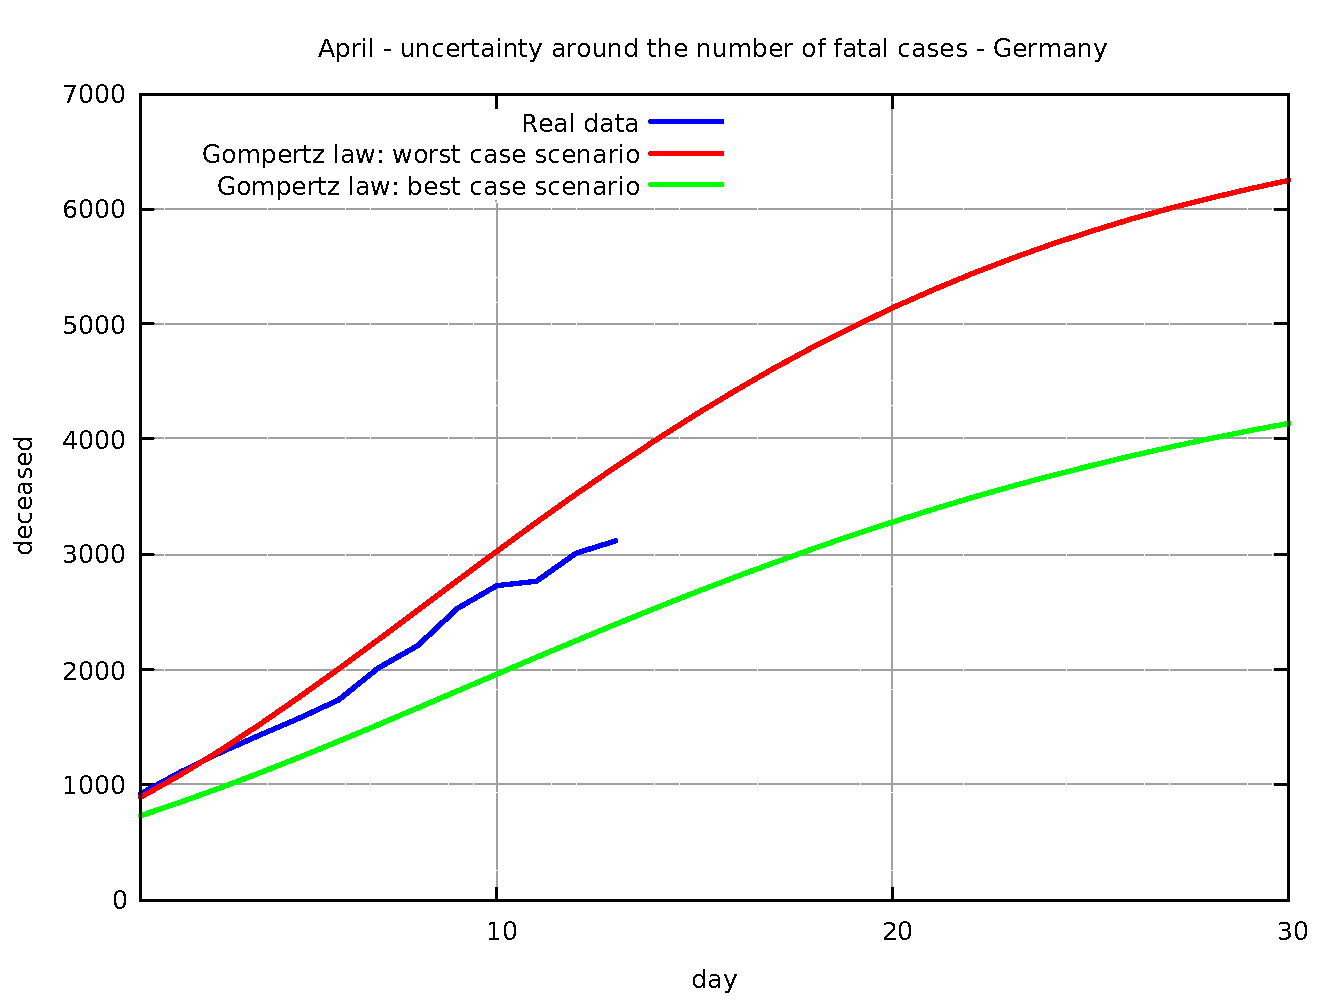
\includegraphics[width=\linewidth]{de_gomp_dead.pdf}
  \caption{Prediction for Germany according to the Gompertz Law}
  \label{fig:boat1}
\end{figure}


\end{document}
